\documentclass[fontsize=11pt]{article}
\usepackage{amsmath}
\usepackage[utf8]{inputenc}
\usepackage[margin=0.75in]{geometry}
\usepackage{graphicx}
\graphicspath{ {./images/} }

\title{CSC110 Project Report: How has climate change affected lyme disease transmission in New York}
\author{Runshi Yang, Haojun Qiu, Chenxu Wang}
\date{Friday, November 6, 2020}

\begin{document}
\maketitle

\section*{Problem Description and Research Question}

The question that our group wants to research on in this project is: \textbf{“how has climate change affected lyme disease transmission around in New York”} As we know, the outbreak of Covid-19 created one of the greatest crises in the global community. While the world is suffering from enormous economic losses, people are also being troubled by both physical and mental agony. This not only raises our concern about viruses themselves and also the adverse impact that climate change could bring to the spread of these viruses. If different climate factors like temperature keep changing in the future, the spread of the diseases can potentially become faster, and they could threaten human health globally.On the other hand, vector-borne diseases could also be affected by climate change since the species that could carry these diseases like mosquitos and ticks tend to live longer in warm weather. With a warmer climate, there could also be more days with high temperature and heavy rainfalls. According to NOAA, the average global temperature has increased at around 0.07 °C per decade$^1$ , and studies have shown that the rainfall rate will increase by around 7\% per increased degree$^4$. They can potentially increase the number of cases and the speed of spreading for different diseases. Therefore, as these are closely related to our health, it is rewarding for us to explore the data from the real world that highly relates to climate change and disease, showing the actual effect through program implementations and reports. 


In our project, we have chosen to look at one specific disease: the lyme disease and predict the effect of climate change on this disease in New York. Therefore, we plan to gather data about the number of virus cases in this region in different years and the possible environmental factors that could cause the rise of the cases. For example, we could gather the data of average monthly temperature in New York and the number of Lyme cases in different months. Then, we want to figure out the effect of each climate factor on the number of disease cases and further, predict future effects based on these data. 

\section*{Dataset Description}

The first set of data that we gathered is the number of lyme disease cases per week in 2016 in different regions and it is from Data.CDC.gov. It is in a csv file, and we have combined it together with some daily weather data in the same area in 2016 in order to match the two data sets. The weather data is also a csv file from Kaggle, which includes information like mean temperature, precipitation, and snowfall. However, not all of the information listed in the data are useful for our calculation. Therefore, we did some filtering process on these two data we’ve collected. For example, the original data of disease cases contain data from different areas across the US, but we only need the data in a small region like New York. Therefore, we have filtered out the data in other regions in our first data. Furthermore, some of the days in our disease data seem to have missing data so we will filter them out as well. Then, we also filter out the snow depth data in our weather data since it is meaningless in the calculation we want to do in later parts. In our project, we plan to predict future data from data in the previous years. Therefore, we have also gathered the disease data in 2014 that has the same format as the disease data in 2016 and apply the same filtering process on it.  We also gathered the monthly weather data in New York like precipitation and mean temperature in 2014 at NOAA in csv files. However, the data that we've gathered are being separated so we also need to do some filtering in order to combine them together. Overall, the data that we will be using in our computation part is our filtered disease data in 2016, filtered climate data in 2016 and the same for data in 2014.\\ 





\section*{Computational Overview}

The first part of our implementation focuses on creating our custom data classes for storing two main types of data that we would be using a lot, which are \texttt{Disease}, and \texttt{Climate}. Having them as custom data class helps us with storing data in natural meaning and will be extra useful if we plan to extend our program to be larger-scaled (Without creating them we could also implement all our functions later on, but we would like to have them for representing data more naturally and meaningfully). Since at the first hand, we thought we would not need to write any method that extended on theses two data classes, so we have harness the python import statement \texttt{from dataclasses import dataclass}, and the python decorator \texttt{@dataclass} to help us with writing the data classes that automatically initialize the instance attributes for us. Before any further exploration, we firstly decided to unify and transform all data in the unit of month, so that later on we would also plot things in month. Thus, for \texttt{Disease}, we have two instance attributes, are \texttt{disease\_name} that refers to the name of the disease as a string, and \texttt{monthly\_cases} that refers to monthly newly added cases as a list of float, (the number of cases is in float since we later on did some arithmetic manipulation to our original data, so it will be represented as float). For \texttt{Climate}, we also have two instance attributes, they are \texttt{monthly\_mean\_temperature} and \texttt{monthly\_sum\_precipitation}, referring to monthly average temperature and total precipitation separately as list of float.


Then, we processed to the implementation of reading and extracting data from our data sets found (in CSV format), and transforming them in the way that we desire them to be (as input of linear regression), for the convenience of our computation later on. In the \texttt{read\_data.py} file, our functions do mainly two things, one is read and extract data from different files we found(the longer part), and the other is further transform the data we extract to what we need as the input for linear regression and plotting (the shorter but "topper-level" one). For the "longer part", we have two main functions, both for reading, extracting and storing data but for different data type - one is called \texttt{extract\_and\_store\_climate\_data} operating on climate data, and the other is called \texttt{extract\_and\_store\_disease\_data} operating on disease data. The input is file name and output are \texttt{Climate} and \texttt{Disease} separately, we also write some helper functions to these two that helps avoid them two be too lengthy, and we also left some comments elaborating what each sub code block of our two main functions does. For the second part, we have five functions that can transform data extracted to the input of our linear regression later on (which means the output of these functions are all list of tuple of float (point)). And the input of these functions are all filenames. One named \texttt{temp\_disease\_list\_2016} transform temperature and disease data into a list tuple, where the first element of the tuple is mean temperature of a certain month in 2016 (the presumed independent variable, in x coordinate), and the second element of the tuple is number of cases added that month (the presumed dependent variable, in y coordinate). And the other three functions called \texttt{prec\_disease\_list\_2016}, \texttt{temp\_disease\_list\_2014},
and \texttt{prec\_disease\_list\_2014} 
have the same type of input and output and similar functionality as \texttt{temp\_disease\_list\_2016}, except that they transform data for different years and dependent variable (precipitation or temperature) as they are named. However, the last one called \texttt{multiple\_2014\_data}, does a slightly different thing - it transforms data to the input of our \textbf{multiple linear regression} later on, which have more than one presumed independent variable, multiple possible determinants (temperatures and precipitations) that possibly affect our presumed dependent variable (cases)). 

 
Finally, the last phase of our computation is doing linear regression and its plotting. For simple linear regression, we wrote them in \texttt{simple\_regression.py} file, and we apply some functions from assignment 1 part 4 to our situation. We have a function named \texttt{simple\_linear\_regression} that returns an estimated value a (represents the slope of the approximated line) and value b (y-intercept) based on the data (list of tuple represented points) as input, which is the basis of our simple linear regression. Then, one of our main and integrated function in this module named \texttt{perform\_regression} that has input named \texttt{train\_data} is a list of points (since we meant to use this function for training data), and the \texttt{xlable} and \texttt{title} that is used for plotting. It calls the above function as helper firstly to calculate a, b values, and the other two helper functions named 
\texttt{plot\_points\_and\_regression} and \texttt{calculate\_r\_squared} to plot the simple linear regression with values a and b, and calculated r squared value afterwards, and then finally, the function returns a tuple in the format of (value a, value b, and r squared). Overall, it does four things: 1) simple linear regression computation, 2) plot the linear regression, and 3) calculate the r squared value, and 4) return a, b, and r squared as a tuple. Another main function in this module named \texttt{predict}, it does the similar thing to \texttt{perform\_regression}, but it works for testing data, and we no longer calculate a, b pair on input data. Instead, we input a, b pair from the result of training data. Then, we also plot line and data points based on this input a, b pair and tested data, and return the r squared value based on it.

For multiple linear regression and its plotting, we have done things differently and use some powerful external libraries to help us implement it, it is written in \texttt{multiple\_regression.py}. We have imported those important modules at the top of the file, they are \texttt{pandas}, \texttt{sklearn}, \texttt{matplotlib}, and \texttt{numpy}. Each of them helps with us in different aspects through out the procedure. For example, the pandas module can help us produce a data frame and the sklearn and matplotlib module can help us to take these data frames and generate a linear regression module from it.  We only have one function in this module named \texttt{multiple\_linear\_regression}. Firstly, we input a dictionary with variable names as keys and list of variable values as values. And then inside the function we use pandas package to convert the input into a dataframe. After that, we use the built in function \texttt{LinearRegression()} to obtain a multiple linear regression model.


\section*{Instruction for obtaining data sets and running program}
\begin{enumerate}
  \item Here are all of the raw data sets that we started with and their url
  
  
  2016 disease data:
  
  https://data.cdc.gov/NNDSS/NNDSS-Table-II-Lyme-disease-to-Meningococcal/93k9-hy54
  
  2016 weather data: 
  
  https://www.kaggle.com/mathijs/weather-data-in-new-york-city-2016?select=weather\_data\_ny\\c\_centralpark\_2016\%281\%29.csv
  
  2014 disease data: 
  
  https://data.cdc.gov/NNDSS/NNDSS-Table-II-Lyme-disease-to-Meningococcal/y6uv-t34t
  
  2014 weather data(precipitation and mean temperature): 
  
  https://www.ncdc.noaa.gov/cag/city/time-series/USW00094728/tavg/all/12/2014-2014 
  
  https://www.ncdc.noaa.gov/cag/city/time-series/USW00094728/pcp/all/12/2014-2014
  
  \item However, we have done some pre-processing of the raw data sets that we find in these websites and all of our computations are done by using data sets that we have filtered. It is available in the link here : 
 
 https://send.utoronto.ca/pickup.php?\\claimID=JDuDXJ5cHGPNaCj9\&claimPasscode=Y6kbzeVykdAiYryC\&emailAddr=runshi.yang\%40mail.utoronto.ca
  
 You may need to enter the following Claim ID and Claim Passcode:

Claim ID: JDuDXJ5cHGPNaCj9

Claim Passcode: Y6kbzeVykdAiYryC


 After downloading our filtered data sets, you should save it in a sub folder called datasets in a Python project. Then install all of the required libraries that we've listed under the requirement.txt file we've submitted along with our functions which are : main.py, data\_class.py, read\_data.py, simple\_regression.py and multiple\_regression.py. \textbf{It is really important that your file path are} datasets/disease\_2014.csv, \newline datasets/disease\_2016.csv,datasets/weather\_2016.csv and datasets/weather\_2014.csv. Other wise, the data might not being read properly. 
 
 \newpage
  
  \item 
  \begin{itemize}
  \item   After you run the first function \texttt{generate\_temp\_lyme\_model()} in main.py in the python console, you will see the output parameter for the first regression model in the console and the following image in the web browser.
  
  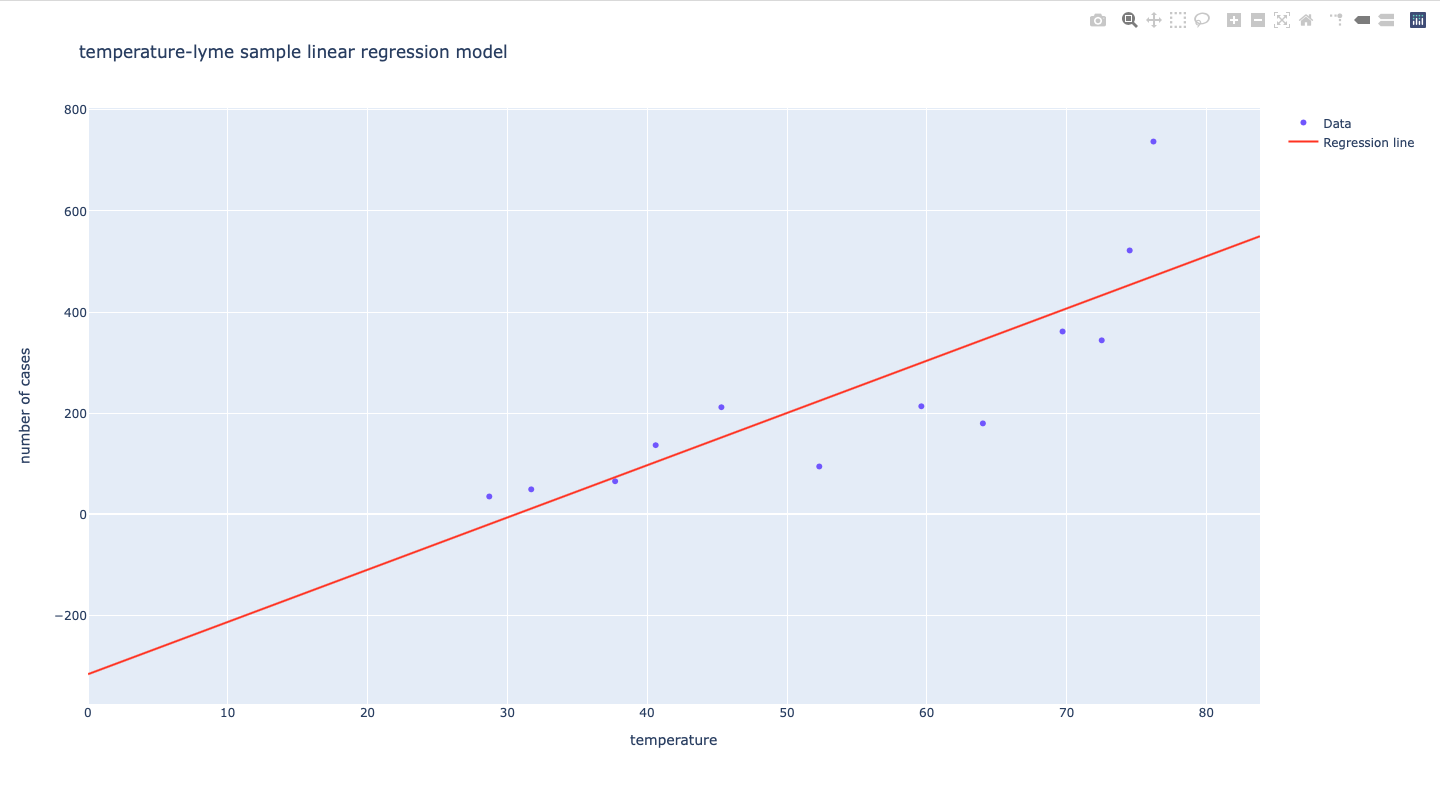
\includegraphics[scale=0.3]{images/image 1.png}
  
  \item After you run the second function \texttt{perform\_temp\_lyme\_prediction()}, you will see the r-squared for the prediction using the first model in the console and the following image in the web browser.
  
  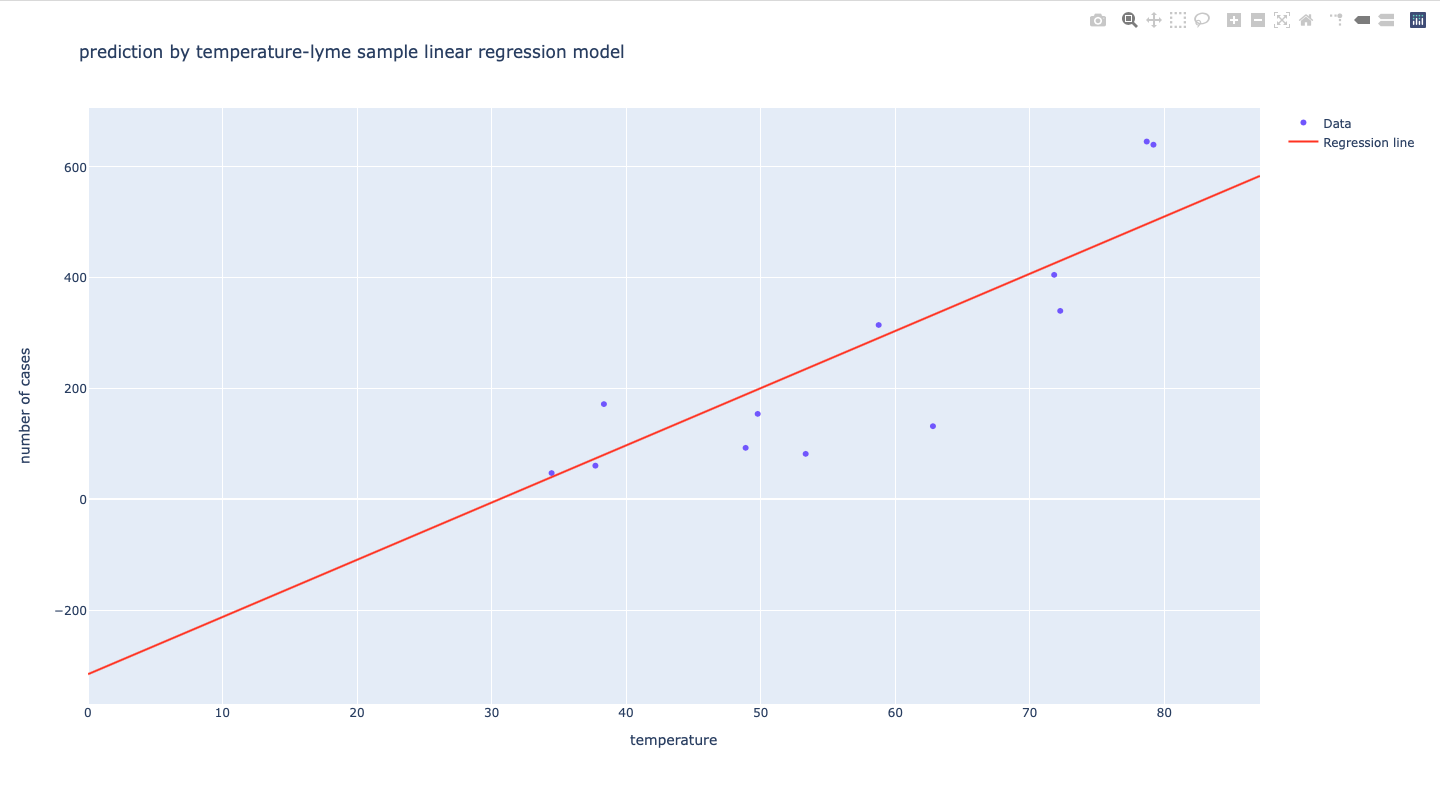
\includegraphics[scale=0.3]{images/image 2.png}
  
  \newpage
  \item After you run the third function \texttt{generate\_prec\_lyme\_model()}, you will see the output parameter for the second regression model in the console and the following image in the web browser.
  
  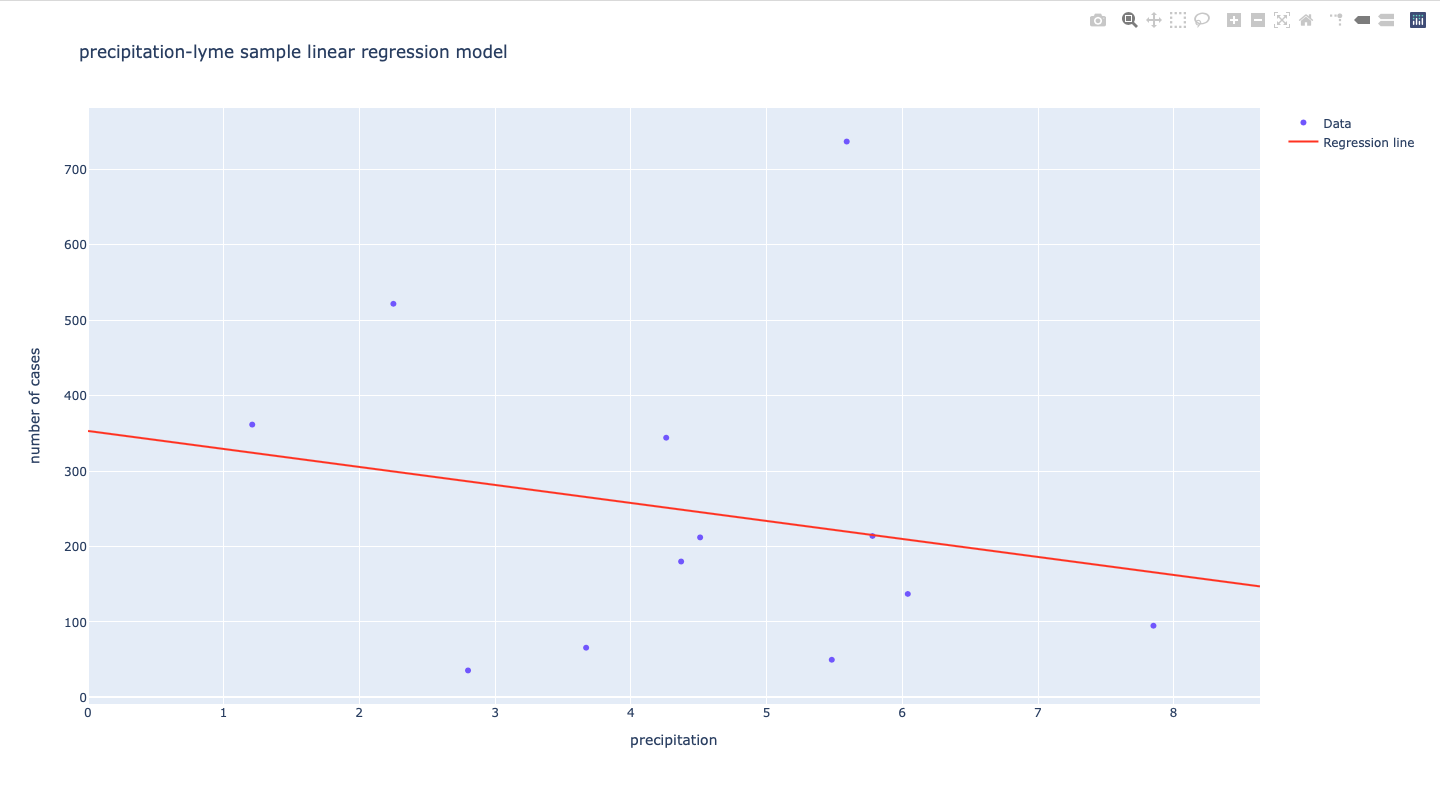
\includegraphics[scale=0.3]{images/image 3.png}
  
  \item After you run the fourth function \texttt{perform\_prec\_lyme\_prediction()}, you will see the r-squared for the prediction using the second model in the console and the following image in the web browser.
  
  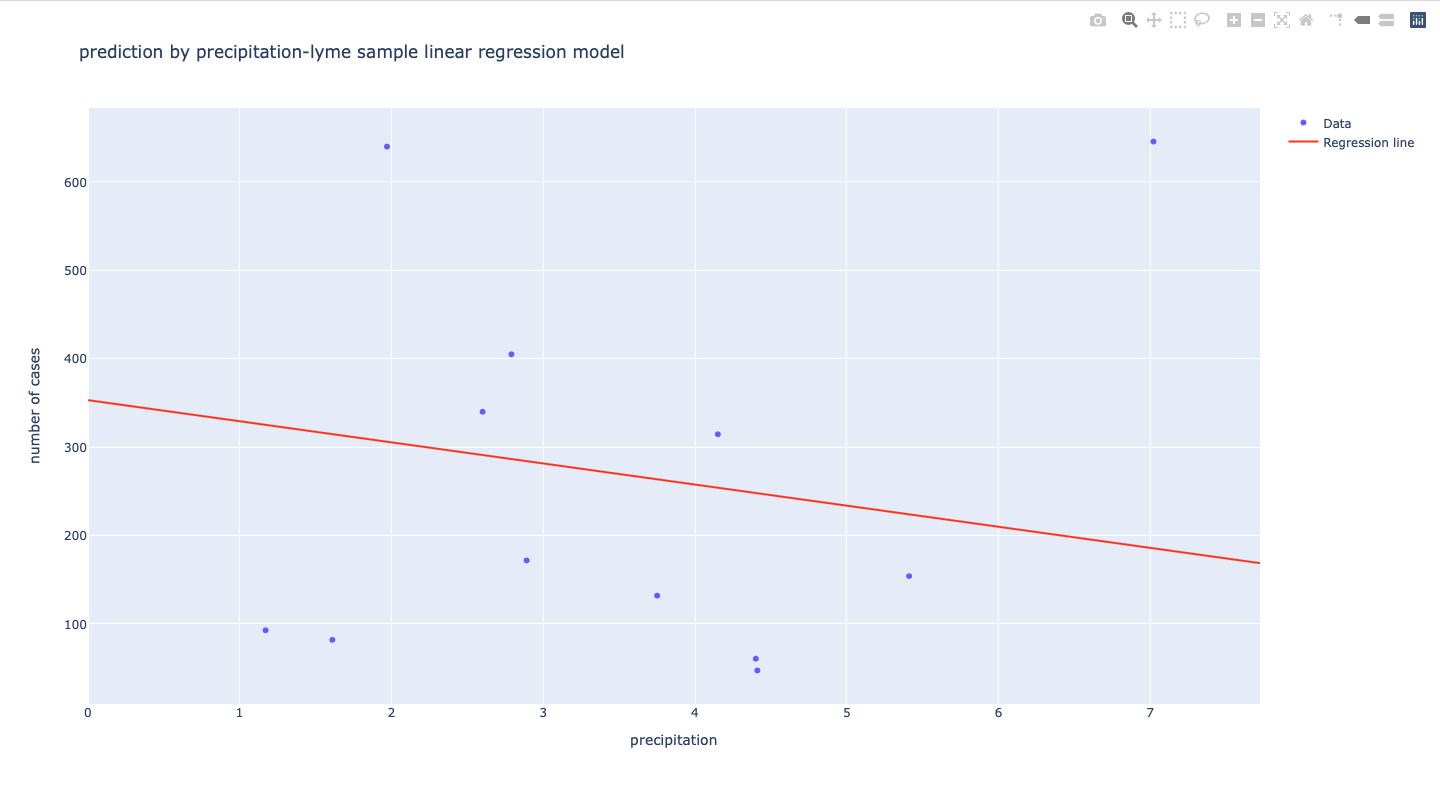
\includegraphics[scale=0.3]{images/image 4.png}
  
  \newpage
  \item After you run the fifth function \texttt{perform\_multiple\_regression(60.0, 1.5)}, you will see the r-squared, adjusted\_r\_squared and coefficients for the multiple linear regression model in the console and the following image.
  
  \centering
  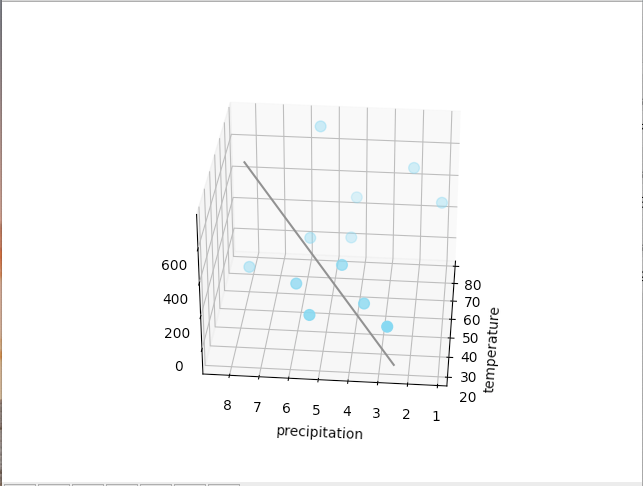
\includegraphics[scale=0.5]{images/image 5.png}
\end{itemize}
  
  
  
  
  
\end{enumerate}


\section*{Changes between plan and final product
}
At the beginning, the question that we plan to work on is "how does environment change affect disease transmission around the world". However, after looking at the feedback from TA, we find out that our original topic is way too general. We should choose a more specific region and disease then study the effect of some environmental factors on that disease. Therefore, we chose a specific disease which is the lyme disease and a smaller region with is New York in our final product. Furthermore, after TA's feedback, we also changed our computation plan. In our new plan, we decided to perform multiple linear regression on the disease data of 2014 and use this result to predict the disease spread of 2016 instead of perform regression on just the data in 2016. The data set description part also changes because of the change in our plan. We managed to find two new data sets which are the climate in New York in 2014 and the number of cases in that year. 


\section*{Discussion Section}

\begin{itemize}
  \item \textbf{Results}

The results of our study help us answer the question of how has climate change affected lyme disease transmission in New York to some extent. When we are analysing the linear association between temperature and number of cases, we built the model as $y_i = 10.32x_i -315.55$, where $y_i$ is the number of cases in the ith month and $x_i$ is the temperature in the ith month. We found that the r-squared of the model we built is 0.71, and we also use it to predict the test data and found r-squared of the prediction is 0.73. So we believe that there is a positive association between temperature and number of cases. However, when we are analysing the linear association between precipitation and number of cases, we found that the r-squared of the model we built is pretty close to 0 (0.04), and when we use the model to predict the test data, the r-squared is negative (-0.12), which means the fit is actually worse than just fitting a horizontal line. So we cannot say there is any linear association between precipitation and number of cases. We think that temperature and precipitation may have a combined effect on lyme transmission, so we did a multiple linear regression using temperature and precipitation as predictors to predict the number of lyme cases and built the model as $z_i = 10.20x_i - 6.23y_i - 281.026$ where $z_i$ is the number of cases in the ith month and $x_i, y_i$ are the temperature and precipitation in the ith month. And the r-squared is about 0.71, which means using both temperature and precipitation to predict the transmission of lyme is relatively accurate.\\
  \item \textbf{Limitations}

The first limitation that we encountered is in our process of reading our data. There are some missing data in our climate data sets that we have filtered out in our first step. However, this might cause the accuracy of our computation part to decrease however it is a limitation that are hard to avoid. Furthermore, In the read data process,we also need to convert our disease data from week into months because our disease data from 2016 and 2014 are both being measured in weeks. To convert them into months, what we plan to do at first is to assume that each month have 28 days so that we can combine the disease data for 4 weeks together into one month. However, the draw back of this approach is that we will end up with 13 months of data since there are 52 weeks of data in total. Therefore, we will have to discard some of the data and our aggression graph would end up being inaccurate. What we did instead is to assume that the number of cases each day are the same and we will have to represent them in floats instead of integers. Then, we transform our data into days first by dividing the number of cases by 7 and multiply them by the number of days in each month. In this approach, we do not need to discard any data from our data sets but the condition that we have to assume is very unlikely to happen in real life. For example, the number of disease cases each day are most likely to be different each day and it will certainly be measured in integers. These assumption will create some errors in our data therefore it is the first limitation that we've encountered. The second limitation we encountered is the effect of other climate factors other than temperature and precipitation. In our project, we considered the climate factors that we think have the most impact on disease transmission which are temperature and precipitation to overcome this limitation. However, some other factors like wind and snow fall are not being considered into our multiple regression graph and they might have some significant impact on the disease we've chosen to explore on.  This is also an important limitation that lowers the accuracy of our computation. \\

  \item \textbf{Further exploration}

Next, we plan to explore more for our project topic, in two dimensions -  breadth and depth.

For breadth, for example, as we discussed above, precipitation is hardly to be convinced as a determinant of the development of the disease. One of our computed r squared shows a negative result, but some others have positive ones, so we could not simply conclude that precipitation is positively correlated with the number of cases. Therefore, I think the first thing we could work on is to explore larger data sets, so we will be able to conclude what kind of correlation that precipitation and cases number of Lyme have (could be some kind of correlation, or possibly not at all linear, or no any correlation), e.g., we can look at years other than 2014 and 2016. Also, for types of disease, we narrowed down our scope to one - Lyme, but we can explore more than one disease. By utilizing functions we have, we are actually only required to find more data sets, and adapt and alter some of the reading and extracting data set functions we have in hand so that they can do the computation that transforms our newly found raw data sets to the input of linear regression. That way, we work on more than one disease, and will possibly have a more powerful conclusion, for example, asserting that the temperature is a significant determinant of deterioration of many types of disease (e.g., COVID-19, what causes our current situation, is a good researched object). Also, we know that there are many factors form what we call climate, so we can study all different factors on diseases, to conclude that what are some most positively/negatively correlated determinants, and also to conclude that what types (the generalized type like infectious disease or hereditary disease) of diseases are influenced by climate as a whole if any, etc. Furthermore, is climate-related with the emergence of new types of disease? We can first do some research and verify what we discovered from our research with our own computations on data sets about the number of newly occurred diseases. Many more potent conclusions we can draw if we start working on more and larger data sets.

For depth, we can extend our ``prediction" part to future years. It is actually the more ``usual" way of prediction done in practice. Firstly, after we have discovered the relation (if linear) between climate factors and the number of cases from past years, we can possibly try to predict the development of some disease in future years by using our result from linear regression, and later on, verify them with upcoming real data sets gathered by others. Also, for the multiple linear regression part, the essence of multiple linear regression is to include multiple (could be more than two) presumed factors at once, but what we have done is only two presumed determinants - precipitation and temperature. So, if we work on more than two factors, we need to think about how to visualize them at once(3D model with 3 axes is not sufficient in the case), as the visualization could be complicated and advanced technique required. 

  \newpage
  \item \textbf{Conclusion}
  
Overall, the conclusion is that there is a positive association between temperature and lyme transmission, while there is no linear association between precipitation and lyme transmission. And  temperature and precipitation have a combined effect on lyme transmission.

\end{itemize}



\section*{References}
\begin{itemize}
  \item [1.] Dahlman, L., \& Lindsey, R. (2020, August 14). Climate Change: Global Temperature: NOAA Climate.gov. Retrieved November 04, 2020, from 

  https://www.climate.gov/news-features/understanding-climate/climate-change-global-temperature
  \item [2.] Hausfather, Z. (2018, January 18). Explainer: What climate models tell us about future rainfall. Retrieved November 04, 2020, from 

  https://www.carbonbrief.org/explainer-what-climate-models-tell-us-about-future-rainfall
  \item[3.] Jordan, R. (2019, March 15). How does climate change affect disease? Retrieved November 04, 2020, from 

  https://earth.stanford.edu/news/how-does-climate-change-affect-disease
  
   \item[4.]Abraham, J. (2017, March 22). Global warming is increasing rainfall rates | John Abraham. Retrieved December 11, 2020, from
   
   
   https://www.theguardian.com/environment/climate-consensus-97-per-cent/2017/mar/22/global-warming-is-increasing-rainfall-rates
\end{itemize}   

\section*{References (data sets)}
\begin{itemize}
 \item NOAA National Centers for Environmental information, Climate at a Glance: City Time Series, published December 2020, retrieved on December 14, 2020 from 
 
 https://www.ncdc.noaa.gov/cag/
 
 \item Waegemakers, M. (2017, September 24). Weather data in New York City - 2016. Retrieved December 14, 2020, from
 
 
 https://www.kaggle.com/mathijs/weather-data-in-new-york-city-2016?select=weatherdatanyccentralpark2016\\\%281\%29.csv
 
 
 \item Centers for Disease control and Prevention, NNDSS - Table II. Lyme disease to Meningococcal - 2014. Retrieved December 14, 2020, from 
 
 https://data.cdc.gov/NNDSS/NNDSS-Table-II-Lyme-disease-to-Meningococcal/y6uv-t34t
 
 \item Centers for Disease control and Prevention, NNDSS - Table II. Lyme disease to Meningococcal - 2016. Retrieved December 14, 2020, from 
 
https://data.cdc.gov/NNDSS/NNDSS-Table-II-Lyme-disease-to-Meningococcal/93k9-hy54
\end{itemize}

\end{document}
